
\documentclass[11pt]{article}
\usepackage{tikz}
\usetikzlibrary{shadows,arrows}
\usepackage{program}
\usepackage{algorithmicx}
\usepackage{algpseudocode}
% Define the layers to draw the diagram
\pgfdeclarelayer{background}
\pgfdeclarelayer{foreground}
\pgfsetlayers{background,main,foreground}
 
% Define block styles  
\tikzstyle{materia}=[draw, fill=blue!20, text width=7.0em, text centered,
  minimum height=1.5em,drop shadow]
\tikzstyle{practica} = [materia, text width=8em, minimum width=10em,
  minimum height=3em, rounded corners, drop shadow]
\tikzstyle{texto} = [above, text width=6em, text centered]
\tikzstyle{linepart} = [draw, thick, color=black!50, -latex', dashed]
\tikzstyle{line} = [draw, thick, color=black!50, -latex']
\tikzstyle{ur}=[draw, text centered, minimum height=0.01em]
 
% Define distances for bordering
\newcommand{\blockdist}{1.3}
\newcommand{\edgedist}{1.5}

\newcommand{\practica}[2]{node (#1) [practica]
  {Pr\'actica #1\\{\scriptsize\textit{#2}}}}


\newcommand{\spacelayer}[3]{node (#1) [practica]
  {#2\\{\scriptsize\textit{#3}}}}


% Draw background
\newcommand{\background}[5]{%
  \begin{pgfonlayer}{background}
    % Left-top corner of the background rectangle
    \path (#1.west |- #2.north)+(-0.5,0.5) node (a1) {};
    % Right-bottom corner of the background rectanle
    \path (#3.east |- #4.south)+(+0.5,-0.25) node (a2) {};
    % Draw the background
    \path[fill=yellow!20,rounded corners, draw=black!50, dashed]
      (a1) rectangle (a2);
    \path (a1.east |- a1.south)+(0.8,-0.3) node (u1)[texto]
      {\scriptsize\textit{#5}};
  \end{pgfonlayer}}

\newcommand{\transreceptor}[3]{%
  \path [linepart] (#1.east) -- node [above]
    {\scriptsize Transreceptor #2} (#3);}



\usepackage{listings}
\usepackage{color}
 
\definecolor{codegreen}{rgb}{0,0.6,0}
\definecolor{codegray}{rgb}{0.5,0.5,0.5}
\definecolor{codepurple}{rgb}{0.58,0,0.82}
\definecolor{backcolour}{rgb}{0.95,0.95,0.92}
 
\lstdefinestyle{mystyle}{
    backgroundcolor=\color{backcolour},   
    commentstyle=\color{codegreen},
    keywordstyle=\color{magenta},
    numberstyle=\tiny\color{codegray},
    stringstyle=\color{codepurple},
    basicstyle=\footnotesize,
    breakatwhitespace=false,         
    breaklines=true,                 
    captionpos=b,                    
    keepspaces=true,                 
    numbers=left,                    
    numbersep=5pt,                  
    showspaces=false,                
    showstringspaces=false,
    showtabs=false,                  
    tabsize=2
}
 
\lstdefinestyle{customset}{   
	backgroundcolor=\color{white},   
    commentstyle=\color{codegreen},
    keywordstyle=\color{magenta},
    stringstyle=\color{codepurple},
    basicstyle=\footnotesize,
    breakatwhitespace=false,         
    breaklines=true,                 
    captionpos=b,                    
    keepspaces=true,    
    showspaces=false,                
    showstringspaces=false,
    showtabs=false,                  
    tabsize=1,
    frame=single,
    numbers=none,
    language=C
}


\lstdefinestyle{customc}{  
  belowcaptionskip=1\baselineskip,
  breaklines=true,
  frame=single,
 % xleftmargin=\parindent,
  language=C,
  showstringspaces=false,
  basicstyle=\footnotesize\ttfamily,
  keywordstyle=\bfseries\color{green!40!black},
  commentstyle=\itshape\color{purple!40!black},
  identifierstyle=\color{blue},
  stringstyle=\color{orange},
  morekeywords={thread, thread_init, thread_exec, join, main},
}

\begin{document}

\title{\vspace{-3.5cm} Implementation designs for fine-grained scheduling in kernel space}


\author{
		 Sreeram Sadasivam\\
		M.Sc Distributed Software Systems\\
		TU Darmstadt, Germany\\
		sreeram.sadasivam@stud.tu-darmstadt.de
}

\date{}


\maketitle

\section*{Design with no checking in user space}

In the following designs, we address the use of check permission of memory access method entirely in Kernel space.

\subsection*{Design with no additional scheduler thread}

The design described in this section addresses the use of no additional scheduler thread. 


\subsubsection*{Trace Registration}

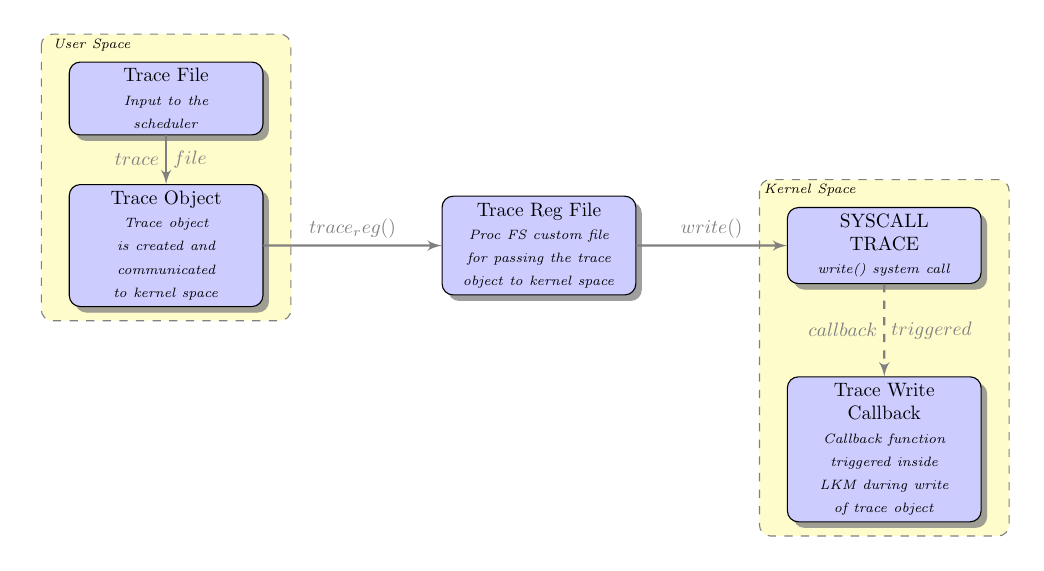
\begin{tikzpicture}[scale=0.7,transform shape]
 
  % Draw diagram elements
  % trace registration area
  \path \spacelayer {TRACEFILE}{Trace File}{Input to the scheduler};  
  \path (TRACEFILE.south)+(0.0,-2.0)\spacelayer {TRACEOBJ}{Trace Object}{Trace object is created and communicated to kernel space};  
  \path (TRACEOBJ.east)+(5.0,0.0) \spacelayer {TRACEPROCFS}{Trace Reg File}{Proc FS custom file for passing the trace object to kernel space};
  \path (TRACEPROCFS.east)+(4.5,0.0) \spacelayer {TRACESYSCALL}{SYSCALL\\ TRACE}{write() system call};  
  \path (TRACESYSCALL.south)+(0.0,-3.0) \spacelayer {TRACECALLBACK}{Trace Write Callback}{Callback function triggered inside LKM during write of trace object};
  
  % Draw arrows between elements

  %thread registration block
  \path [line] (TRACEFILE.south) -- node [left] {$trace$}
									 node [right] {$file$} (TRACEOBJ);
  \path [line] (TRACEOBJ.east) -- node [above] {$trace_reg()$} (TRACEPROCFS);

  \path [line] (TRACEPROCFS.east) -- node [above] {$write()$} (TRACESYSCALL);
  
  \path [linepart] (TRACESYSCALL.south) -- node [left] {$callback$}
                                 node [right]{$triggered$} (TRACECALLBACK);  
  
  %background generation block
  \background{TRACEFILE}{TRACEFILE}{TRACEOBJ}{TRACEOBJ}{User Space}
  \background{TRACESYSCALL}{TRACESYSCALL}{TRACECALLBACK}{TRACECALLBACK}{Kernel Space}

\end{tikzpicture}

The trace file is passed on as an input for the scheduler. 
In the above flow diagram, the trace file is read by the main user thread at the start of its execution. 
It parses the file, creates and passes the trace object to the kernel space as string via a custom file created in the proc file system. 

\subsubsection*{Thread Registration}

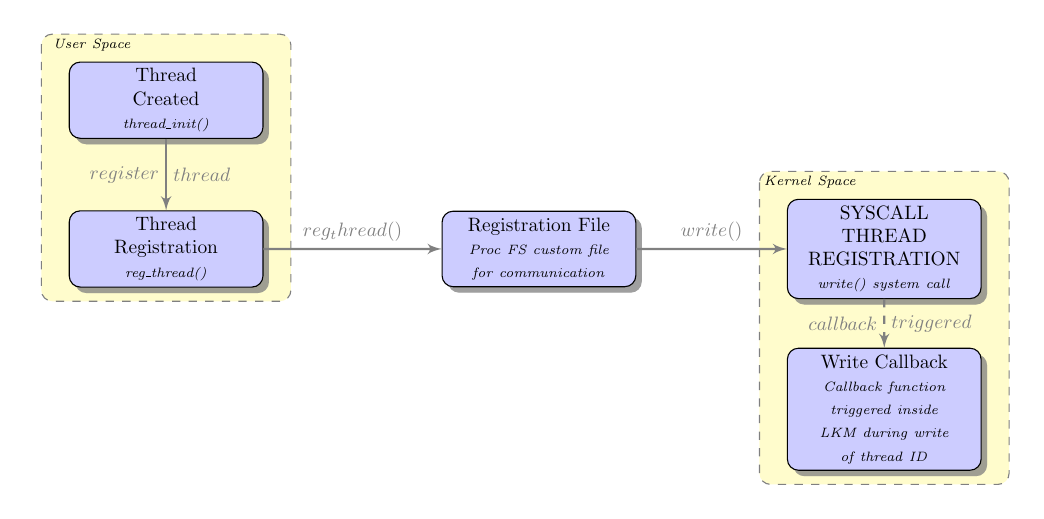
\begin{tikzpicture}[scale=0.7,transform shape] 
  
  % thread registration block area
  \path \spacelayer {THREADINIT}{Thread\\ Created}{thread\_init()};  
  \path (THREADINIT.south)+(0.0,-2.0)\spacelayer {USERTHREADREG}{Thread\\ Registration}{reg\_thread()};  
  \path (USERTHREADREG.east)+(5.0,0.0) \spacelayer {REGPROCFS}{Registration File}{Proc FS custom file for communication};
  \path (REGPROCFS.east)+(4.5,0.0) \spacelayer {REGSYSCALL}{SYSCALL\\ THREAD\\ REGISTRATION}{write() system call};
  \path (REGSYSCALL.south)+(0.0,-2.0) \spacelayer {REGCALLBACK}{Write Callback}{Callback function triggered inside LKM during write of thread ID};

  \background{THREADINIT}{THREADINIT}{USERTHREADREG}{USERTHREADREG}{User Space}
  \background{REGSYSCALL}{REGSYSCALL}{REGCALLBACK}{REGCALLBACK}{Kernel Space}
  
   %Draw arrows between elements
   %thread registration block
  \path [line] (THREADINIT.south) -- node [left] {$register$}
									 node [right] {$thread$} (USERTHREADREG);
  \path [line] (USERTHREADREG.east) -- node [above] {$reg_thread()$} (REGPROCFS);

  \path [line] (REGPROCFS.east) -- node [above] {$write()$} (REGSYSCALL);
  
  \path [linepart] (REGSYSCALL.south) -- node [left] {$callback$}
                                 node [right]{$triggered$} (REGCALLBACK);

\end{tikzpicture}

In the above picture, the registration block happens when a user thread is created. 
The registration happens via a custom proc file system. 




\subsubsection*{Memory Assessment}

Prior to any global memory access, the given design would invoke \emph{IOCTL} command with \emph{CTXT\_SWITCH} and thread id of the thread which addressed the memory event as its parameters. 


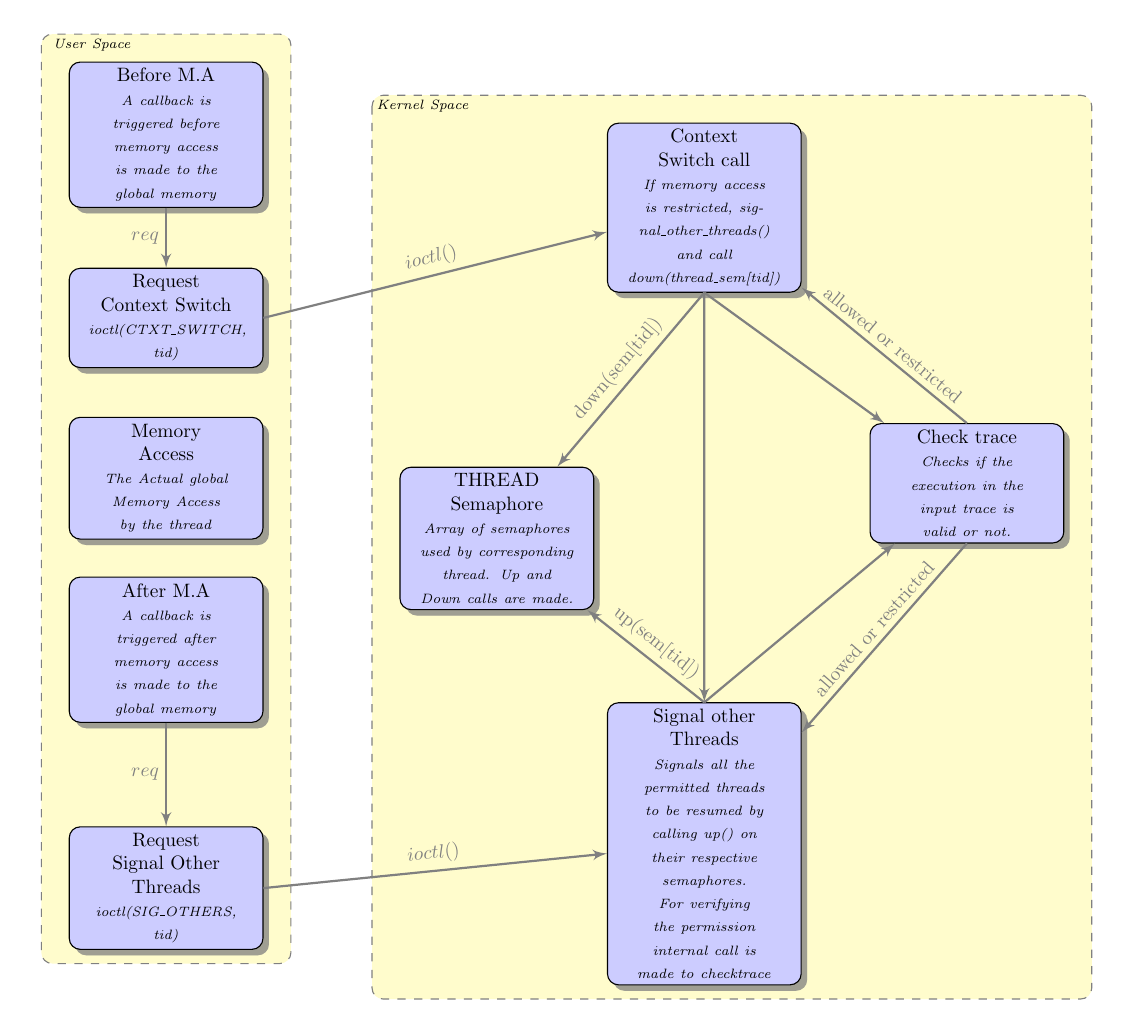
\begin{tikzpicture}[scale=0.7,transform shape]
 
 
  % memory assessment area
  
  \path \spacelayer {BEFOREMA}{Before M.A}{A callback is triggered before memory access is made to the global memory};
  \path (BEFOREMA.south)+(0.0,-2.0) \spacelayer {REQCTXTSWITCH}{Request \\ Context Switch}{ioctl(CTXT\_SWITCH, tid)};
  
  \path (REQCTXTSWITCH.south)+(0.0,-2.0) \spacelayer {MEMACCESS}{Memory\\ Access}{The Actual global Memory Access by the thread};

  \path (MEMACCESS.south)+(0.0,-2.0) \spacelayer {AFTERMA}{After M.A}{A callback is triggered after memory access is made to the global memory};
  \path (AFTERMA.south)+(0.0,-3.0) \spacelayer {USRSIGOTHERS}{Request \\ Signal Other Threads}{ioctl(SIG\_OTHERS, tid)};  
  
  
  \path (REQCTXTSWITCH.east)+(8.0,2.0) \spacelayer {CONTEXTSWITCH}{Context Switch call}{If memory access is restricted, signal\_other\_threads() and call down(thread\_sem[tid]) }; 
  \path (CONTEXTSWITCH.east)+(3.0,-5.0) \spacelayer {CHECKTRACE}{Check trace}{Checks if the execution in the input trace is valid or not.}; 
  \path (CONTEXTSWITCH.west)+(-2.0,-6.0) \spacelayer {THREADSEM}{THREAD\\ Semaphore}{Array of semaphores used by corresponding thread. Up and Down calls are made.}; 
 \path (CONTEXTSWITCH.south)+(0.0,-10.0) \spacelayer {SIGNALOTHERS}{Signal other\\ Threads}{Signals all the permitted threads to be resumed by calling up() on their respective semaphores. For verifying the permission internal call is made to checktrace}; 
 
  
  

  % Draw arrows between elements

 
 
  

  %memory assessment block
  \path [line] (BEFOREMA.south) -- node [left] {$req$} (REQCTXTSWITCH);
  \path [line] (AFTERMA.south) -- node [left] {$req$} (USRSIGOTHERS);

  \path [line] (REQCTXTSWITCH.east) -- node [midway,above,sloped] {$ioctl()$} (CONTEXTSWITCH);
  
  \path [line] (CONTEXTSWITCH.south) -- node [left] {} (CHECKTRACE);
  \path [line] (CONTEXTSWITCH.south) -- node [midway,above,sloped] {down(sem[tid])} (THREADSEM);
  \path [line] (CONTEXTSWITCH.south) -- node [left] {} (SIGNALOTHERS);
  \path [line] (CHECKTRACE.north) -- node [midway,above,sloped] {allowed\ or\ restricted} (CONTEXTSWITCH);  
   
  \path [line] (SIGNALOTHERS.north) -- node [left] {} (CHECKTRACE);   
  \path [line] (CHECKTRACE.south) -- node [midway,above,sloped] {allowed\ or\ restricted} (SIGNALOTHERS);
  \path [line] (SIGNALOTHERS.north) -- node [midway,above,sloped] {up(sem[tid])} (THREADSEM);
   
   \path [line] (USRSIGOTHERS.east) -- node [midway,above,sloped] {$ioctl()$} (SIGNALOTHERS);
  %\path [linepart] (CONTEXTSWITCH.west) -- node [above] {$thread$}
                                 %node [right]{$resume$} (THREADRESUME);

  %background generation block
 
  \background{BEFOREMA}{BEFOREMA}{USRSIGOTHERS}{USRSIGOTHERS}{User Space}
  \background{THREADSEM}{CONTEXTSWITCH}{CHECKTRACE}{SIGNALOTHERS}{Kernel Space}
  

\end{tikzpicture}


\newpage
\subsubsection*{Pseudo Implementation}
\begin{lstlisting}[title=Data Types Section used by user space and kernel space, style=customc]
enum IOCTL CMDS  { 
	GET_CURR_CLK = 1, 
  	CTXT_SWITCH = 2, 
  	SIGNAL_OTHER_THREADS = 3,
  	RESET_CLK = 4,
  	SET_MY_CLK = 5
}
enum  mem_access{
	e_ma_restricted = 0,
	e_ma_allowed 	= 1
} 
struct vec_clk {
	int clocks[THREAD_COUNT],
}
struct trace_node {
	thread_id_t tid;
	vec_clk clk;
	int valid;
}

struct trace {
	trace_nodes trace_obj_arr[TRACE_LIMIT];
}
\end{lstlisting}

\begin{lstlisting}[title=Check Permission for memory access, style=customc]
mem_access check_mem_acc_perm(vec_clk* curr_vec_clk, vec_clk* trace_inst, thread_id_t tid) {

   int i;
   if(trace_inst->clocks[tid-1] == curr_vec_clk->clocks[tid-1]) 
   {
     for i in range(0, THREAD_COUNT) 
     {
	if(i!=(tid-1)) 
	{
	 if(trace_inst->clocks[i] <= curr_vec_clk->clocks[i]) 
	 {
	 	continue;
	 }
	 else 
	 {
	 	return e_ma_restricted;
	 }
	}
     }
   }
   else if(trace_inst->clocks[tid-1] < curr_vec_clk->clocks[tid-1]) 
   {
   	return e_ma_restricted;
   }
   return e_ma_allowed;
}

\end{lstlisting}


\begin{lstlisting}[title=User Space Implementation, style=customc]
BeforeMA() {	
	ioctl(CTXT_SWITCH, thread_id);	
}

AfterMA() {	
	ioctl(SIGNAL_OTHER_THREADS, thread_id);
}

reset_clock() {
	ioctl(RESET_CLK);
}

//This method is defined by the thread library which is used by the user
thread_create_impl(thread t) {
	t ->thread_init(tid);
	t ->thread_exec(thread_function);
}

thread_function() {
	reg_thread();	//This method increments a threadcount variable in kernel space.
	....	
	Before_MA(); 	//function triggered before accessing the global memory
	Mem_Access();   //global memory access permitted for the thread
	AfterMA();		//function triggered after accessing the global memory		
	....
	thread_exit()
}

trace_reg() {	
	fd = open("/proc/trace_reg",O_RDWR);
	close(fd);	
}

main() {	
	trace_reg()
	thread t = thread_create(tid, thread_function); 
	//thread_create_impl() is called internally
	.....
	t.join();	
	return EXIT_SUCCESS;
}


\end{lstlisting}
\begin{lstlisting}[title=Kernel Space - General module definitions, style=customc]
semaphore threads_sems[THREAD_COUNT];
int wait_queue[THREAD_COUNT];
trace trace_obj;
vec_clk curr_clk;
int thread_count = 0;

module_init() {
	for i in range(0,THREAD_COUNT) {
		init(threads_sem[i] = 0;
		wait_queue[i] = 0;
		curr_clk[i] = 0;
	}
	alloc_ioctl_device();//method used to allocate ioctl device.
}

trace_reg_callback() {
	//The method parses the trace which is passed as string and stores in trace_obj
}

reg_thread_callback() {
	thread_count++;
}

\end{lstlisting}
\newpage
\begin{lstlisting}[title=Kernel Space - IOCTL, style=customc]
/* This method is triggered whenever ioctl commands are issued from the user space */
ioctl_access(IOCTL_CMDS cmd) {	
	switch(cmd) {
		case CTXT_SWITCH: 
			req_ctxt_switch(thread_id);//requests for context switch
			break;
		case SIGNAL_OTHER-THREADS:
			Increment_curr_clk(thread_id); //this will increment the current clk for the given thread id.
			signal_all_other_threads(thread_id);
			break;
		case GET_CURR_CLK:
			get_curr_clk();//returns the current vector clock.
			break;
		case RESET_CLK:
			reset_clk(); //reset the current vector clock to zero.
			break:		
		case SET_CURR_CLK:
			set_curr_clk(clk);//sets the current vector clock with the clk received.
	}
}

//Methods of interest with respect to the ioctl cmds
mem_access check_mem_access_with_trace(thread_id_t tid) {
	...
	//method internally calls check_mem_acc_perm() with current clock time and uses the first valid instance vector clock registered for a given thread in the trace array.
		
	//returns e_ma_allowed|e_ma_restricted based on the check_mem_acc_perm()
}

void ctxt_switch_thread(thread_id_t tid) {	
	down(threads_sem[tid-1]); //perform semaphore down operation respective semaphore.
	/**if the value is already 0 when performing the down, the thread waits until the value is positive.*/
}

void signal_all_other_threads(thread_id_t tid) {
	//critical section for wait queue
	for i in(0,THREAD_COUNT) {
		if(i!=(tid-1)) {
			if(check_mem_access_with_trace(i+1) == e_ma_allowed) {
				/**Performs up operation on the respective thread semaphore.*/
				up(threads_sem[i]);
				wait_queue[i]=0;			
			}		
		}
	}	
	
	//critical section ends.
}

void req_ctxt_switch(thread_id_t tid) {
		if(check_mem_access_with_trace(tid) == e_ma_restricted) {

		signal_all_other_threads(tid);
		
		//critical section for waitqueue
		wait_queue[tid-1] = 1; //sets the thread inline for waiting
		//critical section ends.
		
		ctxt_switch_thread(tid);

	}
}

\end{lstlisting}


\subsection*{Design with an additional scheduler thread}

In this design we create an additional scheduler thread primarily addressing the signaling mechanism pertained in the previous design. 
By having an additional scheduler thread, we move the entire signaling system to the scheduler thread.
Thus, reducing the execution overhead encountered in the user space thread for signaling other threads.

The major change from the previous design apart from additional thread is in the memory assessment block.

\subsubsection*{Memory assessment block}
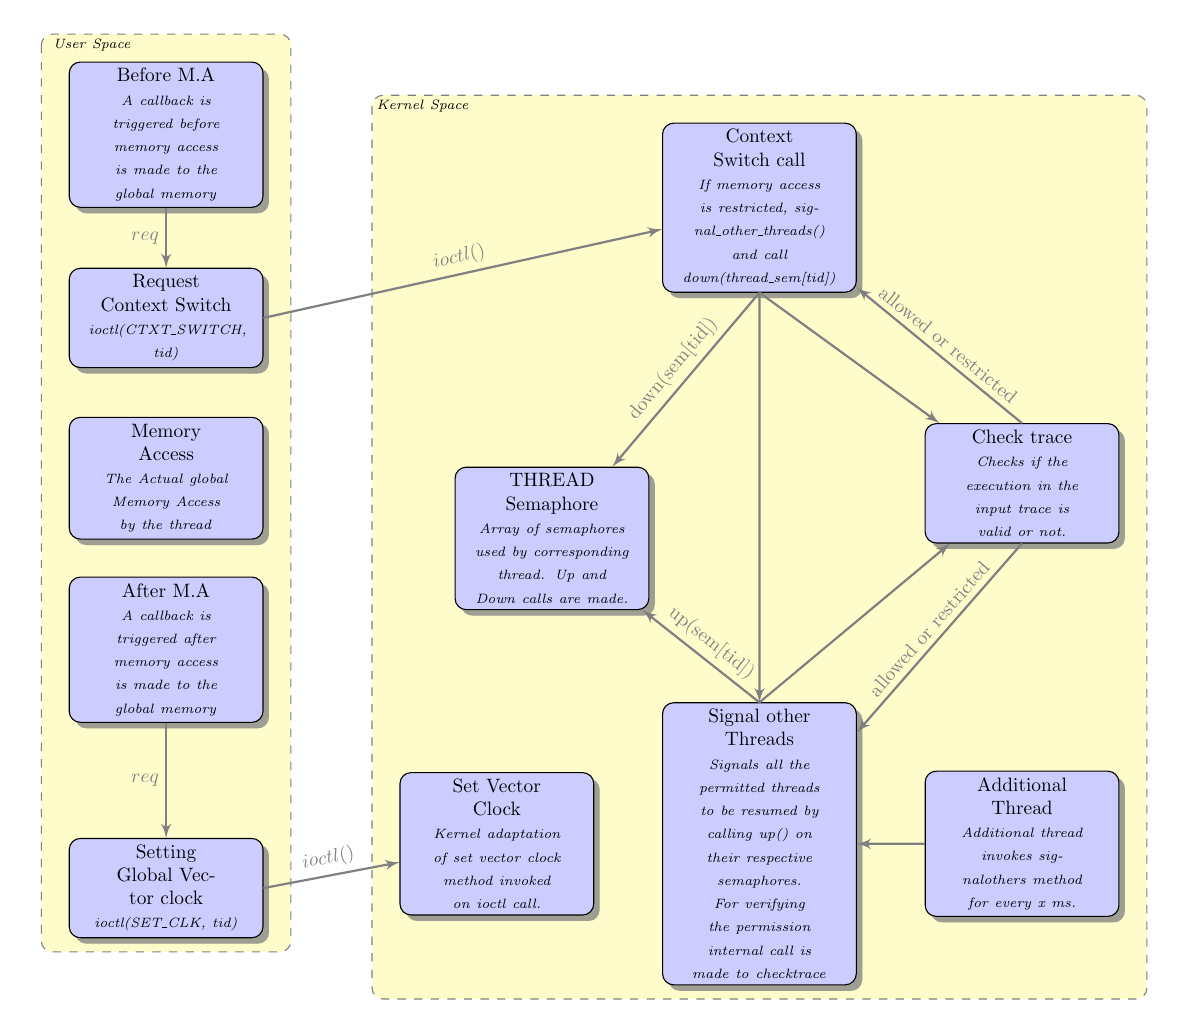
\begin{tikzpicture}[scale=0.7,transform shape]
 
 
  % memory assessment area
  
  \path \spacelayer {BEFOREMA}{Before M.A}{A callback is triggered before memory access is made to the global memory};
  \path (BEFOREMA.south)+(0.0,-2.0) \spacelayer {REQCTXTSWITCH}{Request \\ Context Switch}{ioctl(CTXT\_SWITCH, tid)};
  
  \path (REQCTXTSWITCH.south)+(0.0,-2.0) \spacelayer {MEMACCESS}{Memory\\ Access}{The Actual global Memory Access by the thread};

  \path (MEMACCESS.south)+(0.0,-2.0) \spacelayer {AFTERMA}{After M.A}{A callback is triggered after memory access is made to the global memory};
  \path (AFTERMA.south)+(0.0,-3.0) \spacelayer {SETCLK}{Setting \\ Global Vector clock}{ioctl(SET\_CLK, tid)};  
  
  
  \path (REQCTXTSWITCH.east)+(9.0,2.0) \spacelayer {CONTEXTSWITCH}{Context Switch call}{If memory access is restricted, signal\_other\_threads() and call down(thread\_sem[tid]) }; 
  \path (CONTEXTSWITCH.east)+(3.0,-5.0) \spacelayer {CHECKTRACE}{Check trace}{Checks if the execution in the input trace is valid or not.}; 
  \path (CONTEXTSWITCH.west)+(-2.0,-6.0) \spacelayer {THREADSEM}{THREAD\\ Semaphore}{Array of semaphores used by corresponding thread. Up and Down calls are made.}; 
  \path (CONTEXTSWITCH.south)+(0.0,-10.0) \spacelayer {SIGNALOTHERS}{Signal other\\ Threads}{Signals all the permitted threads to be resumed by calling up() on their respective semaphores. For verifying the permission internal call is made to checktrace}; 
 \path (SIGNALOTHERS.west)+(-3.0,0.0) \spacelayer {SETVECCLK}{Set Vector\\ Clock}{Kernel adaptation of set vector clock method invoked on ioctl call.}; 
 \path (SIGNALOTHERS.east)+(+3.0,0.0) \spacelayer {ADDTHREAD}{Additional\\ Thread}{Additional thread invokes signalothers method for every x ms.};  
  

  % Draw arrows between elements

 
 
  

  %memory assessment block
  \path [line] (BEFOREMA.south) -- node [left] {$req$} (REQCTXTSWITCH);
  \path [line] (AFTERMA.south) -- node [left] {$req$} (SETCLK);

  \path [line] (REQCTXTSWITCH.east) -- node [midway,above,sloped] {$ioctl()$} (CONTEXTSWITCH);
  
  \path [line] (CONTEXTSWITCH.south) -- node [left] {} (CHECKTRACE);
  \path [line] (CONTEXTSWITCH.south) -- node [midway,above,sloped] {down(sem[tid])} (THREADSEM);
  \path [line] (CONTEXTSWITCH.south) -- node [left] {} (SIGNALOTHERS);
  \path [line] (CHECKTRACE.north) -- node [midway,above,sloped] {allowed\ or\ restricted} (CONTEXTSWITCH);  
   
  \path [line] (SIGNALOTHERS.north) -- node [left] {} (CHECKTRACE);   
  \path [line] (CHECKTRACE.south) -- node [midway,above,sloped] {allowed\ or\ restricted} (SIGNALOTHERS);
  \path [line] (SIGNALOTHERS.north) -- node [midway,above,sloped] {up(sem[tid])} (THREADSEM);
   
   \path [line] (SETCLK.east) -- node [midway,above,sloped] {$ioctl()$} (SETVECCLK);
  %\path [linepart] (CONTEXTSWITCH.west) -- node [above] {$thread$}
                                 %node [right]{$resume$} (THREADRESUME);
   \path [line] (ADDTHREAD.west) -- node [left] {} (SIGNALOTHERS);
  %background generation block
 
  \background{BEFOREMA}{BEFOREMA}{SETCLK}{SETCLK}{User Space}
  \background{SETVECCLK}{CONTEXTSWITCH}{CHECKTRACE}{SIGNALOTHERS}{Kernel Space}
  

\end{tikzpicture}
\newpage
\subsubsection*{Pseudo Implementation}

The major changes are in kernel space code. 
However, there are minor variations in the AfterMA() in user space. 

\begin{lstlisting}[title=User Space Implementation, style=customc]
//Rest of the code remains the same

AfterMA() {	
	ioctl(SET_MY_CLK, thread_id);
}

//Rest of the code remains the same

\end{lstlisting}

\begin{lstlisting}[title=Kernel Space - General module definitions, style=customc]
//code remains the same

void signal_permitted_threads() {
	//critical section for wait queue
	for i in(0,THREAD_COUNT) {
		if(wait_queue[i] == 1) {
			if(check_mem_access_with_trace(i+1) == e_ma_allowed) {
				/**Performs up operation on the respective thread semaphore.*/
				up(threads_sem[i]);
				wait_queue[i]=0;			
			}		
		}
	}	
	
	//critical section ends.
}

module_init() {
	//code remains the same
	
	kernel_thread tk = create_kernel_thread(signal_permitted_threads)
	tk->setTimerCallForEvery(x) //this method will make call to signal permitted threads for every x ms.
}

//code remains the same
\end{lstlisting}

\section*{Design with checking in user space}

In the following designs, we address the use of check permission of memory access method both in User Space and Kernel space.

\subsection*{Design with no additional scheduler thread}

//more to come

\subsection*{Design with an additional scheduler thread}
//more to come

%
%\begin{tikzpicture}[scale=0.7,transform shape]
% 
%  % Draw diagram elements
%  % trace registration area
%  \path \spacelayer {TRACEFILE}{Trace File}{Input to the scheduler};  
%  \path (TRACEFILE.south)+(0.0,-2.0)\spacelayer {TRACEOBJ}{Trace Object}{Trace object is created and communicated to kernel space};  
%  \path (TRACEOBJ.east)+(5.0,0.0) \spacelayer {TRACEPROCFS}{Trace Reg File}{Proc FS custom file for passing the trace object to kernel space};
%  \path (TRACEPROCFS.east)+(4.5,0.0) \spacelayer {TRACESYSCALL}{SYSCALL\\ TRACE}{write() system call};  
%  \path (TRACESYSCALL.south)+(0.0,-3.0) \spacelayer {TRACECALLBACK}{Trace Write Callback}{Callback function triggered inside LKM during write of trace object};
%  
%  % Draw arrows between elements
%
%  %thread registration block
%  \path [line] (TRACEFILE.south) -- node [left] {$trace$}
%									 node [right] {$file$} (TRACEOBJ);
%  \path [line] (TRACEOBJ.east) -- node [above] {$trace_reg()$} (TRACEPROCFS);
%
%  \path [line] (TRACEPROCFS.east) -- node [above] {$write()$} (TRACESYSCALL);
%  
%  \path [linepart] (TRACESYSCALL.south) -- node [left] {$callback$}
%                                 node [right]{$triggered$} (TRACECALLBACK);  
%  
%  %background generation block
%  \background{TRACEFILE}{TRACEFILE}{TRACEOBJ}{TRACEOBJ}{User Space}
%  \background{TRACESYSCALL}{TRACESYSCALL}{TRACECALLBACK}{TRACECALLBACK}{Kernel Space}
%
%\end{tikzpicture}
%
%The trace file is passed on as an input for the scheduler. 
%In the above flow diagram, the trace file is read by the main user thread at the start of its execution. 
%It parses the file, creates and passes the trace object to the kernel space as string via a custom file created in the proc file system. 
%
%\begin{tikzpicture}[scale=0.7,transform shape] 
%  
%  % thread registration block area
%  \path \spacelayer {THREADINIT}{Thread\\ Created}{thread\_init()};  
%  \path (THREADINIT.south)+(0.0,-2.0)\spacelayer {USERTHREADREG}{Thread\\ Registration}{reg\_thread()};  
%  \path (USERTHREADREG.east)+(5.0,0.0) \spacelayer {REGPROCFS}{Registration File}{Proc FS custom file for communication};
%  \path (REGPROCFS.east)+(4.5,0.0) \spacelayer {REGSYSCALL}{SYSCALL\\ THREAD\\ REGISTRATION}{write() system call};
%  \path (REGSYSCALL.south)+(0.0,-2.0) \spacelayer {REGCALLBACK}{Write Callback}{Callback function triggered inside LKM during write of thread ID};
%
%  \background{THREADINIT}{THREADINIT}{USERTHREADREG}{USERTHREADREG}{User Space}
%  \background{REGSYSCALL}{REGSYSCALL}{REGCALLBACK}{REGCALLBACK}{Kernel Space}
%  
%   %Draw arrows between elements
%   %thread registration block
%  \path [line] (THREADINIT.south) -- node [left] {$register$}
%									 node [right] {$thread$} (USERTHREADREG);
%  \path [line] (USERTHREADREG.east) -- node [above] {$reg_thread()$} (REGPROCFS);
%
%  \path [line] (REGPROCFS.east) -- node [above] {$write()$} (REGSYSCALL);
%  
%  \path [linepart] (REGSYSCALL.south) -- node [left] {$callback$}
%                                 node [right]{$triggered$} (REGCALLBACK);
%
%\end{tikzpicture}
%
%In the above picture, the registration block happens when a user thread is created. 
%The registration happens via a custom proc file system. 
%
%
%
%
%\section*{Memory Assessment Block}
%
%\begin{tikzpicture}[scale=0.7,transform shape]
% 
% 
%  % memory assessment area
%  
%  \path \spacelayer {BEFOREMA}{Before M.A}{A callback is triggered before memory access is made to the global memory};
%  \path (BEFOREMA.south)+(0.0,-2.0) \spacelayer {MEMASSESSMENT}{Memory\\ Assessment}{Checks if the memory access is permitted or not using trace object};
%  \path (MEMASSESSMENT.south)+(0.0,-2.0) \spacelayer {SCHEDYIELD}{Scheduler\\ yield}{scheduler\_yield()};
%  
%  \path (SCHEDYIELD.south)+(0.0,-4.0) \spacelayer {THREADRESUME}{Thread\\ Resume}{The thread which started the context switch is resumed if the trace permits its execution otherwise, another thread is resumed based on the trace.};
%  
%  \path (SCHEDYIELD.east)+(10.0,0.0) \spacelayer {CONTEXTSWITCH}{Context Switch call}{Function internally performs verification by calling check\_trace() again inside kernel space. And then performs the actual context switch}; 
%  \path (CONTEXTSWITCH.south)+(0.0,-2.0) \spacelayer {CHECKTRACE}{Check trace}{Checks if the execution in the input trace is valid or not.}; 
%  \path (CONTEXTSWITCH.north)+(0.0,3.0) \spacelayer {MAPDATASTRUCTURE}{MAP\\ UTID to TaskID }{Data structure which has a map for Task ID to every UTID};
%  
%  
%
%  % Draw arrows between elements
%
% 
% 
%  
%
%  %memory assessment block
%  \path [line] (BEFOREMA.south) -- node [left] {$Check$}
%						     node [right] {$Trace$} (MEMASSESSMENT);
%
%  \path [line] (MEMASSESSMENT.south) -- node [left] {$Not$}
%						     node [right] {$Permitted$} (SCHEDYIELD);
%
%  \path [line] (SCHEDYIELD.east) -- node [above] {$context\_switch(UTID)$} (CONTEXTSWITCH);
%  
%  \path [line] (CONTEXTSWITCH.south) -- node [left] {$check\_trace()$} (CHECKTRACE);
%  
%  \path [line] (CONTEXTSWITCH.north) -- node [left] {$taskID\_for\_utid(UTID)$} (MAPDATASTRUCTURE);
%
%  \path [linepart] (CONTEXTSWITCH.west) -- node [above] {$thread$}
%                                 node [right]{$resume$} (THREADRESUME);
%
%  %background generation block
% 
%  \background{BEFOREMA}{BEFOREMA}{THREADRESUME}{THREADRESUME}{User Space}
%  \background{MAPDATASTRUCTURE}{MAPDATASTRUCTURE}{CHECKTRACE}{CHECKTRACE}{Kernel Space}
%  
%
%\end{tikzpicture}
%
%
%In the memory assessment block, the user thread initially performs a check of permissions to access memory. 
%The check happens with the help of the trace object created from the trace input file. 
%The memory assessment block is involved whenever there is a global memory event. 
%Based on the assessment in kernel space, the assessment thread is resumed or another thread which was paused would be resumed. 


\end{document} 